\subsection{Lepton charge mis-identification}
\subsubsection*{Mechanisms}
The misidentification rate of leptons is governed by \\
\begin{align}
-\langle\frac{dE}{dx}\rangle \varpropto \frac{E}{m^2}
\end{align}
Thus this rate is significant for electrons and high energy ($E > 400GeV$) muons. Therefore only the electron charge misidentification is calculated. \\

Electron charge misidentification is due to:
\begin{enumerate}
\item Bremsstrahlung photon and conversion electron
\item Track misidentification
\end{enumerate}

Since a magnetic field exists within the detector, it is possible to infer the charge and momentum of electrons by the curvature of their tracks. However, there are cases when the reconstruction gives the wrong charge. 

\begin{figure}[h]
\centering
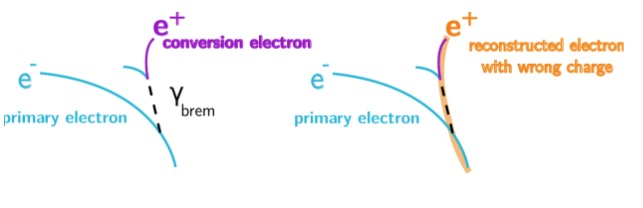
\includegraphics[width=\textwidth]{ChargeMisID/Brem}
\caption[Electron charge misidentification by bremsstrahlung]{Bremsstrahlung}
\label{fig:brem}
\end{figure}
\begin{figure}[h]
\centering
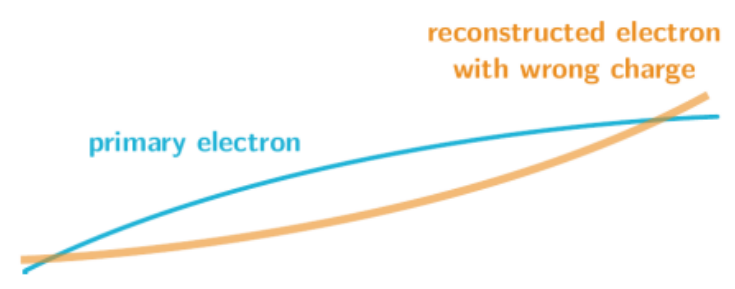
\includegraphics[width=\textwidth]{ChargeMisID/WrongTrack}
\caption[Electron charge misidentification by track mis-reconstruction]{Track mis-reconstruction}
\label{fig:wrong-track}
\end{figure}

\underline{Bremsstrahlung} \\
Charge misidentification may occur when an electron radiates a photon early in the detector (in the beampipe, or the first layers of the inner tracker). The radiated photon may then undergo pair production, and the converted electrons would leave tracks in the inner tracker.  One of these wrong tracks may then be matched to an energy deposit inside the calorimeter. In case the electron that left the track has the opposite charge to the original, then the charge inferred would be opposite to the charge of the original electron \cite{ElectronReco2011}. (Figure \ref{fig:brem}). 

The probability of bremsstrahlung increases with the amount of material the electron interacts with. Hence as the material budget of the detector changes with $|\eta|$ (Figure \ref{fig:material-budget}), it is expected that the charge misidentification rate ought to depend on  $|\eta|$.

\begin{figure}[h]
\centering
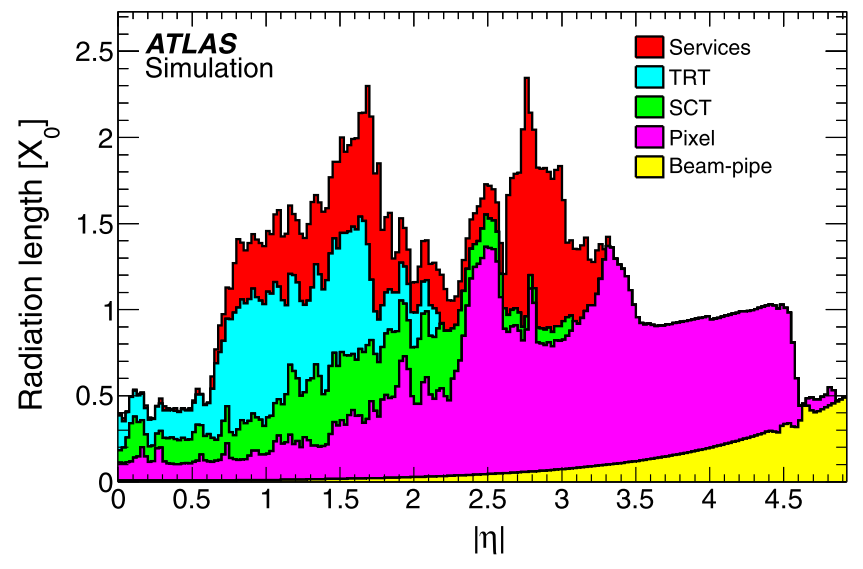
\includegraphics[scale=0.4]{ChargeMisID/Material-budget.png}
\caption[Amount of material traversed by a particle as a function of $|\eta|$]{Amount of material in front of the solenoid magnet and EM calorimeters traversed by a particle as a function of $|\eta|$. Figure from \cite{ElectronReco2011}.}
\label{fig:material-budget}
\end{figure}

\underline{Track mis-reconstruction}\\
Another possible source of charge misidentification is track mis-reconstruction. The near straight track of a high $p_T$ electron may be reconstructed with the opposite curvature, thus giving the opposite sign. (Figure \ref{fig:wrong-track})

\subsubsection*{Likelihood Method for Measuring Charge misID}
$Z\rightarrow e^\pm e^\mp$ events are studied for its relatively clean signal (see Figure \ref{fig:mll_ee_OS}) and because, by charge conservation,  the two daughter electrons of the $Z$ must be of opposite sign. In principle, if a $Z\rightarrow e^\pm e^\pm$ event is found, it must the case that the charge of one electron has been misidentified. The likelihood method was used to measure the charge misidentification rate. An alternative method, the tag-and-probe method, was also attempted; the results obtained were unsatisfactory. 

\begin{figure}[h]
\centering
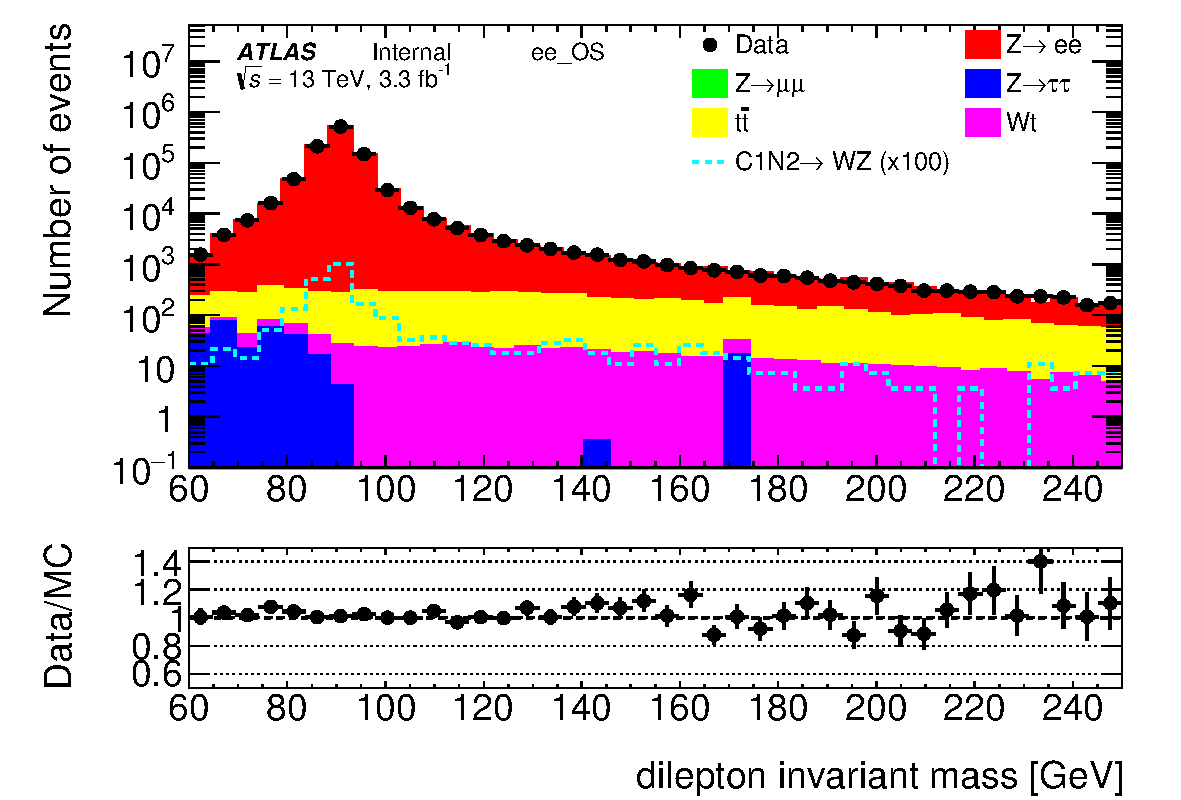
\includegraphics[scale=0.6]{ChargeMisID/mll_ee_OS.pdf}
\caption[Distribution of opposite-sign dielectron events]{Distribution of opposite-sign dielectron events. Note that the region near the Z mass $(91.2\ GeV)$ the signal is dominated by $Z\rightarrow e^\pm e^\mp$ events by at least 2 orders of magnitude. Plot by Lo Cheuk Yee, HKU.}
\label{fig:mll_ee_OS}
\end{figure}

The most likely rate of charge misidentification is determined by extremizing a likelihood function. 

$Z\rightarrow ee$ events were selected by imposing the following cuts:
\begin{itemize}
\item Events with two electrons
\item $80\ GeV < m_{ee} < 100\ GeV$
\item Both same-sign and opposite-sign events are selected
\end{itemize}

The probability of observing a same sign event is:
\begin{equation}
p = P(e_1 \text{ correct sign})P(e_2 \text{ wrong sign}) + P(e_1 \text{ wrong sign})P(e_2 \text{ correct sign})
\end{equation}

Each electron is assigned a bin which depends on its $|\eta|$ and $p_T$. For events where one electron falls into bin $i$ and the other electron falls into bin $j$, the probability of observing a same-sign event is: 
\begin{equation}
p =(1-\epsilon_i)\epsilon_j + (1-\epsilon_j)\epsilon_i
\end{equation}
where $\epsilon_i$ is the charge misidentification rate in bin $i$.

The expected number of same-sign events is given by
\begin{equation}
N^{exp}_{SS} = np 
\end{equation}

A binomial distribution of observing $nss$ same-sign events is expected:
\begin{equation}
P(nss |\epsilon_i, \epsilon_j) =  C^n_{nss} p^{nss}(1-p)^{n-nss}
\end{equation}

Since $p$ is small, this can be approximated well by a Poisson distribution: 
\begin{equation}
P(nss |\epsilon_i, \epsilon_j) = \frac{(N^{exp}_{SS})^{nss} e^{-N^{exp}_{SS}}}{nss!}
\end{equation}

With this equation of the probability of observing $nss$ same-sign events given $\epsilon_i$ and $\epsilon_j$, the likelihood function of having $\epsilon_i$, $\epsilon_j$ given $nss$ observed same-sign events can be defined: 
\begin{equation}
L(\epsilon_i, \epsilon_j | nss) \equiv P(nss |\epsilon_i, \epsilon_j)
\end{equation}

For the likelihood across all combinations of bins $i,j$,
\begin{equation}
\mathcal{L} = \prod\nolimits_{i,j} L(\epsilon_i, \epsilon_j)
\end{equation}

By maximizing the likelihood function, the most probable $\epsilon_i$, $\epsilon_j$ can be found for a given $nss$ observed same sign events. To simplify calculation, the logarithm function is applied to $\mathcal{L}$. To take advantage of the minimizer in ROOT, the negative of the function is minimized. 

The final function to be minimized is 

\begin{equation}
-\ln \mathcal{L} = -\sum\nolimits_{i,j} \Big\{ {nss}_{ij} \ln\big(n_{ij}[\epsilon_j(1-\epsilon_i) + \epsilon_i(1-\epsilon_j)]\big) - n_{ij}[\epsilon_j(1-\epsilon_i) + \epsilon_i(1-\epsilon_j)] - \ln (nss_{ij}!) \Big\}
\end{equation} 

The bins in which the rates are calculated are defined in table \ref{table:binning}.

\begin{table}[h!]
\centering
\begin{tabular}{c | c}
\textbf{Variable} & \textbf{Bin edges} \\
\hline
$|\eta|$ & 0, 0.5, 1, 1.37, 1.52, 1.8, 2.0, 2.5 \\
$p_T$ (GeV) &  20, 30, 40, 50, 60, 80, 120, 1000
\end{tabular}
\caption{Binning in $|\eta|$ and $p_T$}
\label{table:binning}
\end{table}

\subsubsection*{Validation with Monte Carlo}
A Monte Carlo (MC) sample of simulated $Z \rightarrow ee$ events\footnote{MC sample used: \texttt{mc15\_13TeV.361106.PowhegPythia8EvtGen\_AZNLOCTEQ6L1\_Zee.merge.DAOD\_SUSY2. e3601\_s2576\_s2132\_r7725\_r7676\_p2666}}  was used to develop and validate the likelihood algorithm. The information saved in the MC sample includes the \textit{truth} information of the simulated events, and the reconstructed event information produced from a detector simulator. 

For every reconstructed electron selected by the aforementioned conditions, an attempt was made to find the charge of the original daughter electron of Z. A reconstructed electron was first matched to a truth particle with the smallest $\Delta R = \sqrt{\Delta \phi^2 + \Delta \eta^2} < 0.1$ separation from the reconstructed electron. The truth particle was rejected if it was not an electron.\footnote{It could be the case that a hadron was misidentified as an electron \cite{ElectronReco2011}.} The decay path was then traversed upwards to find the original daughter electron of a Z boson. The truth particle was rejected if no Z boson was found in the path, or if the daughter particle of Z was not an electron.\footnote{It was found that sometimes the algorithm would match to a final-state radiation photon from Z.} An example of this algorithm is shown in Figure \ref{fig:find-daughter-electron}. This algorithm does not work on \textsc{Sherpa} samples because information about the Z is not saved. The sample used for this study was generated by \textsc{Powheg}. 

\begin{figure}[h!]
\centering
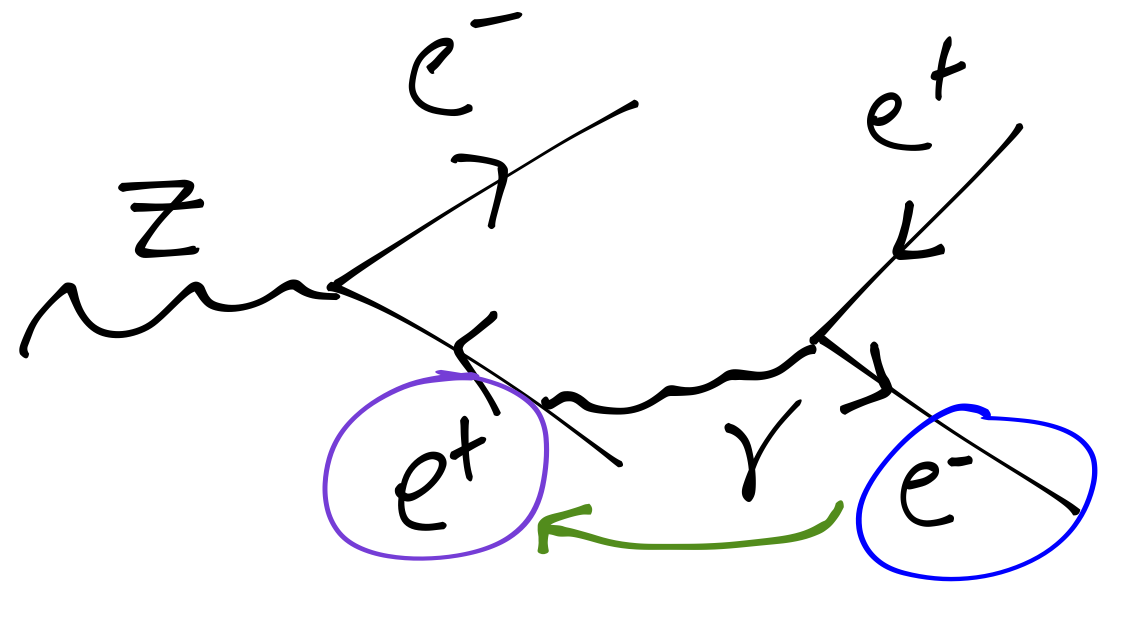
\includegraphics[scale=0.35]{ChargeMisID/MC-truth}
\caption[Finding the original daughter electron of Z]{Finding the  daughter electron of Z. The electron circled in blue is the truth electron matched to the reconstructed electron. The decay was traversed upwards to find the original daughter electron of a Z boson, circled in purple.}
\label{fig:find-daughter-electron}
\end{figure}

If the original electron daughter of Z was found, then it was considered to be the \textit{matched} electron of the reconstructed electron. If the charge of the matched electron was not identical to the charge of the reconstructed electron, then the charge was considered to be misidentified. Thus the true charge misidentification rate in each bin can be defined as:

\begin{equation}
\epsilon_{\text{MC}} = \frac{\text{Number of reconstructed electrons with charge opposite to its matched electron}}{\text{Total number of matched electrons}}
\end{equation}

The rates obtained in MC from the likelihood method and the truth are compared in figure \ref{fig:MCrates}. See figure \ref{fig:2DMC} for full 2D histograms.

\begin{figure}[h]
\centering
\includegraphics[page=1,scale=0.35]{ChargeMisID/1007-MC-comparison/EtaPt.pdf}
\includegraphics[page=2,scale=0.35]{ChargeMisID/1007-MC-comparison/EtaPt.pdf}\\
\includegraphics[page=3,scale=0.35]{ChargeMisID/1007-MC-comparison/EtaPt.pdf}
\includegraphics[page=4,scale=0.35]{ChargeMisID/1007-MC-comparison/EtaPt.pdf}\\
\includegraphics[page=5,scale=0.35]{ChargeMisID/1007-MC-comparison/EtaPt.pdf}
\includegraphics[page=6,scale=0.35]{ChargeMisID/1007-MC-comparison/EtaPt.pdf}
\end{figure}

\begin{figure}[h]
\ContinuedFloat
\centering
\includegraphics[page=7,scale=0.35]{ChargeMisID/1007-MC-comparison/EtaPt.pdf}
\caption{Comparison of rates in MC obtained from truth and likelihood method for signal electrons}
\label{fig:MCrates}
\end{figure}

\begin{figure}[h]
\begin{subfigure}[t]{\textwidth}
\centering
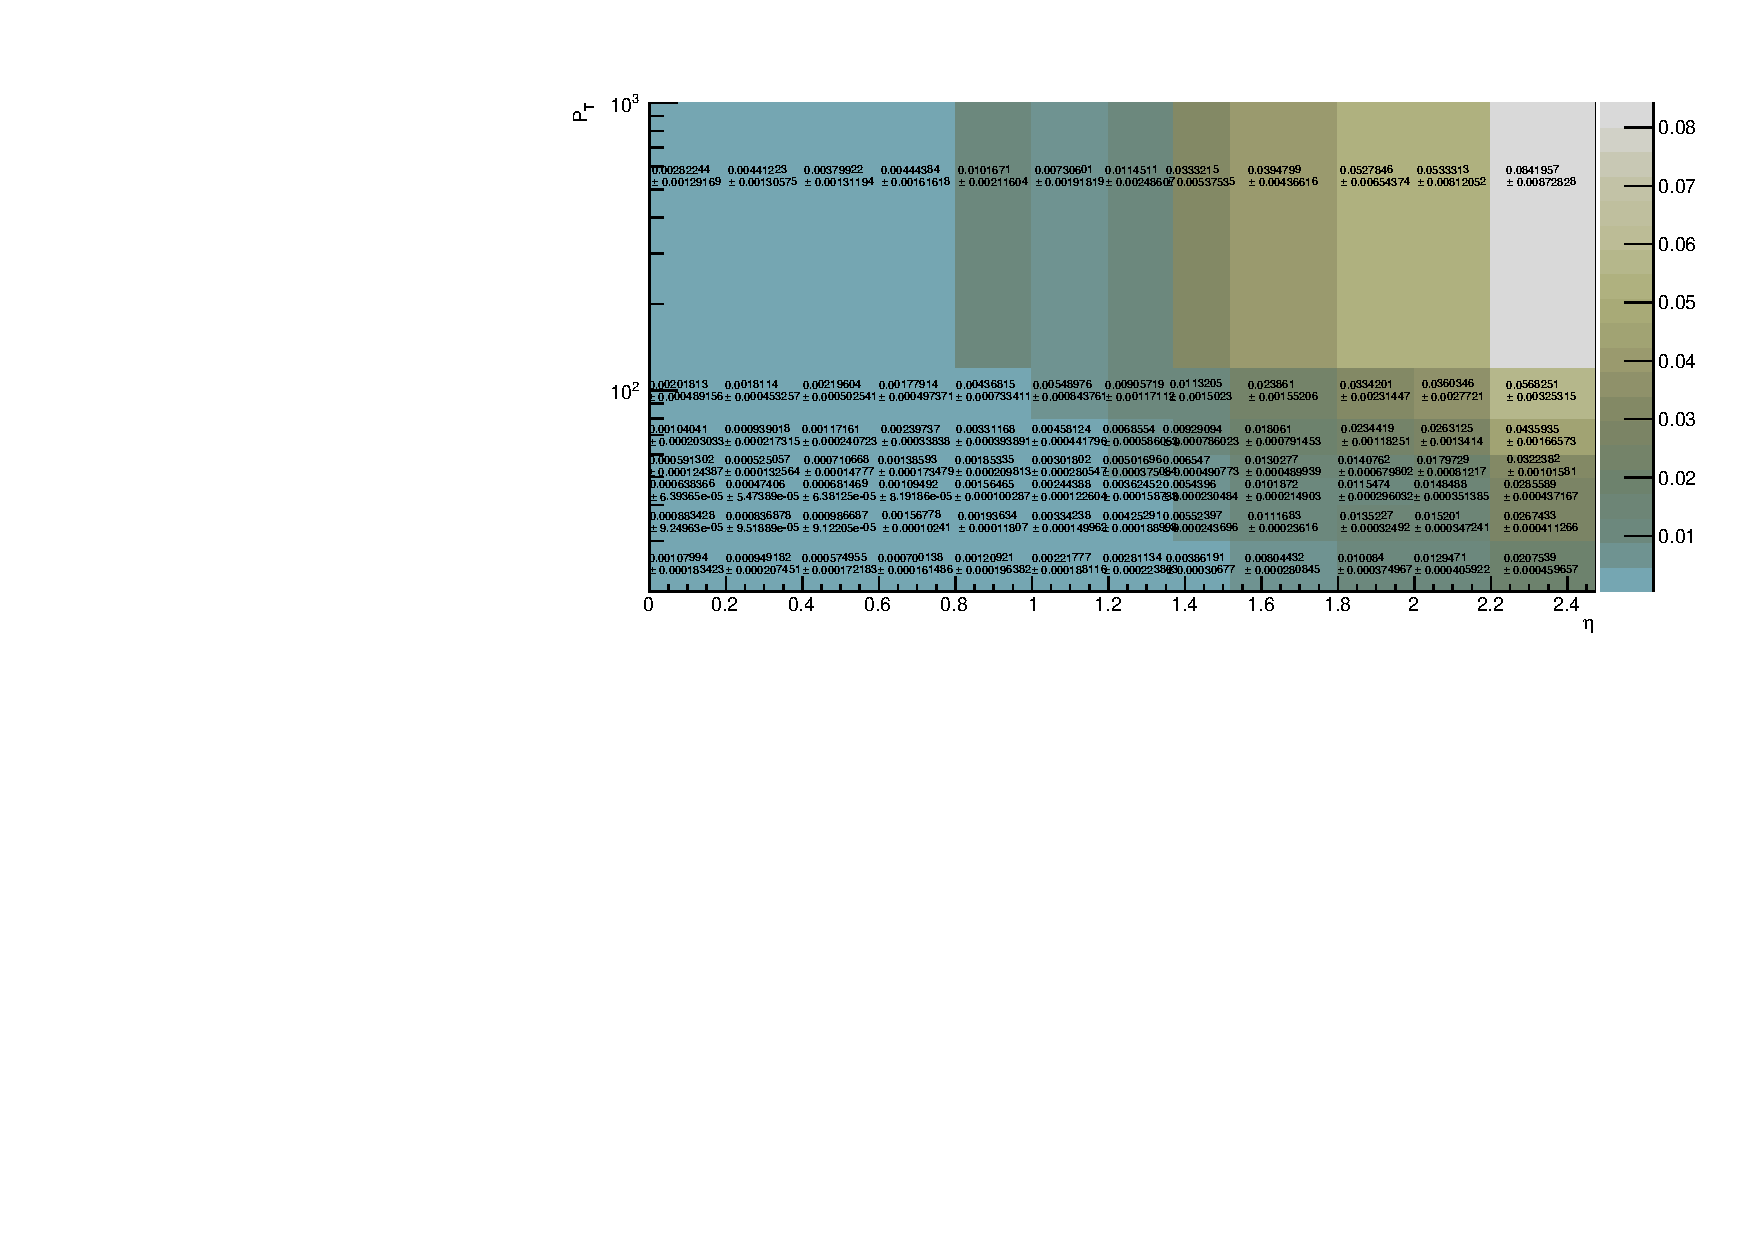
\includegraphics[width=\textwidth]{ChargeMisID/dataRates/MCLH}
\caption{Rates from likelihood method}
\end{subfigure}
\end{figure}

\begin{figure}[h]
\ContinuedFloat
\centering
\begin{subfigure}[t]{\textwidth}
\centering
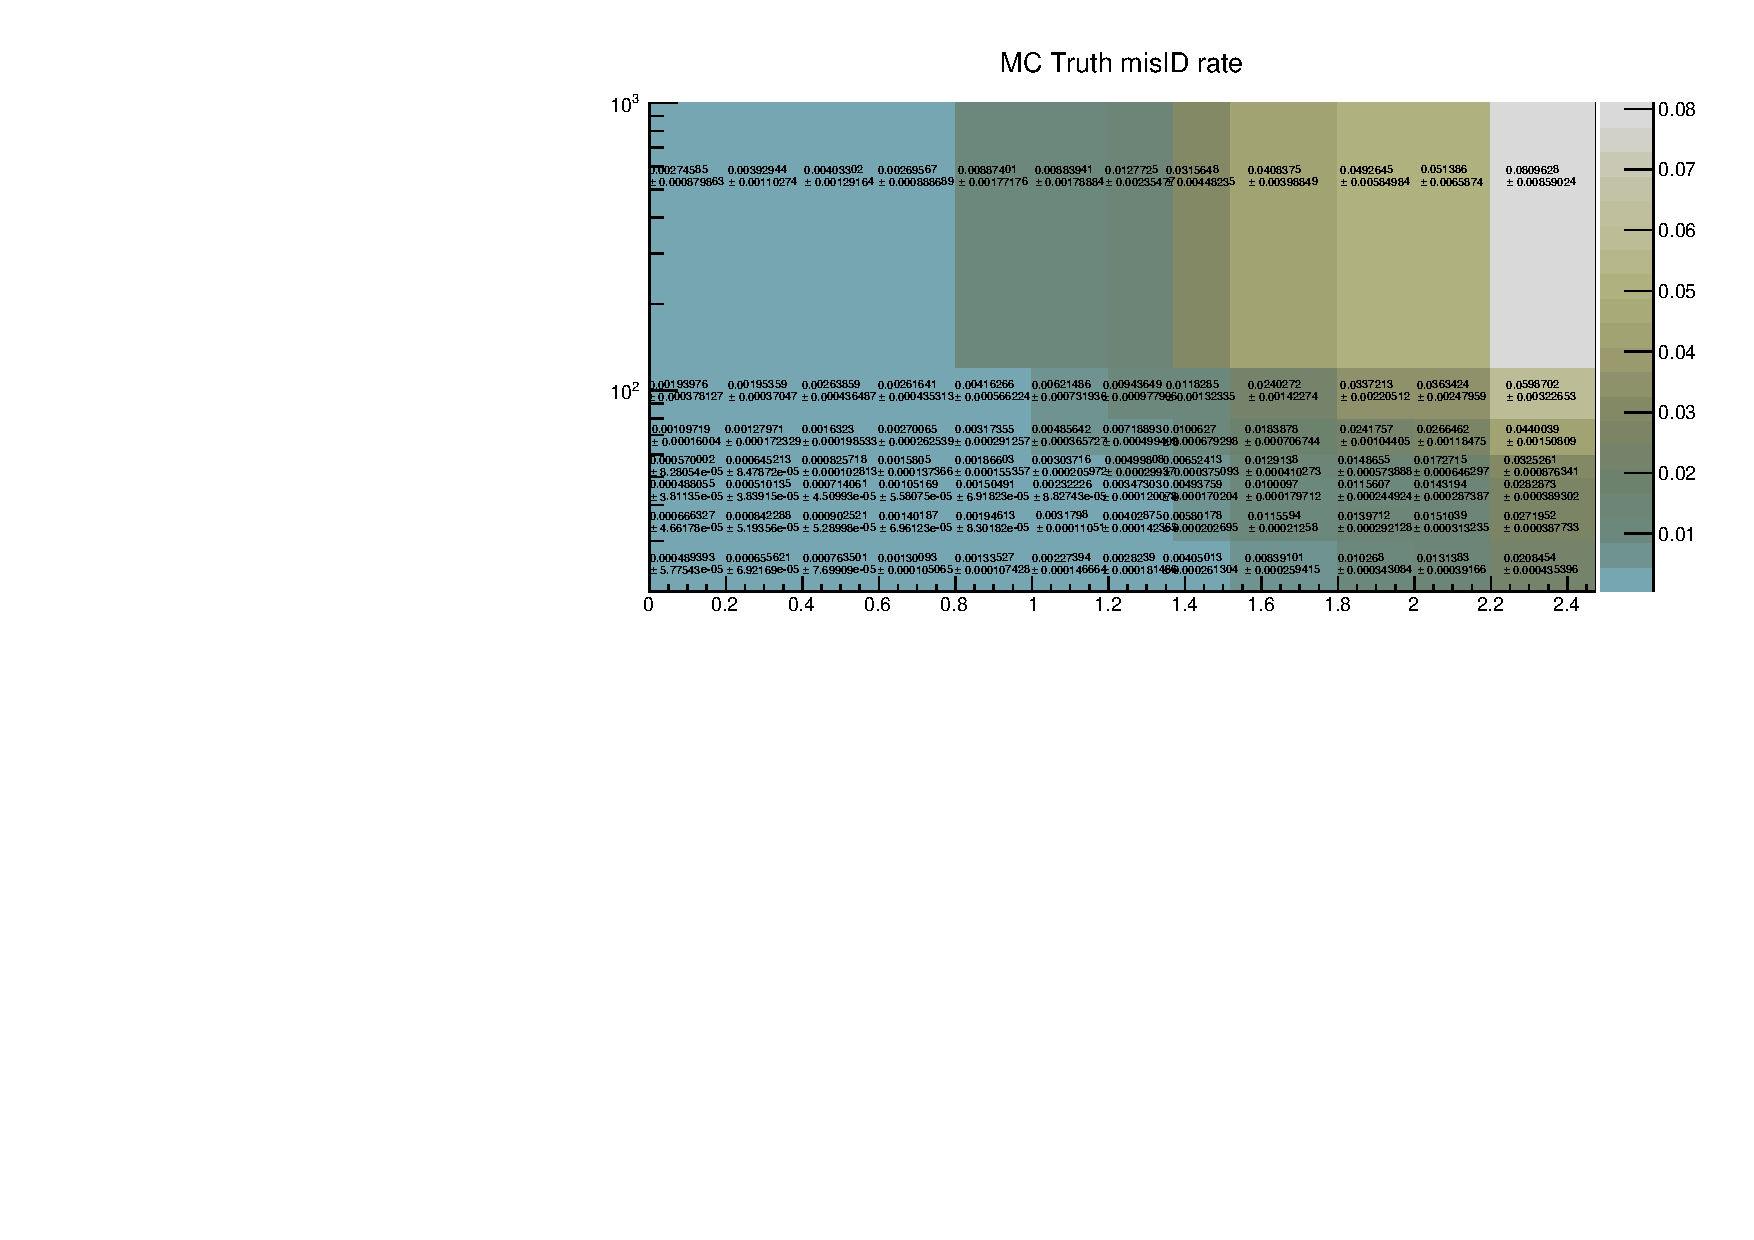
\includegraphics[width=\textwidth]{ChargeMisID/dataRates/MCtruth}
\caption{Rates from MC truth}
\end{subfigure}
\caption{Rates from $Z\rightarrow ee$ MC}
\label{fig:2DMC}
\end{figure}

\FloatBarrier
\subsubsection*{\pT correction}
In the $Z\rightarrow ee$ MC sample, the same-sign distributions can be estimated from the opposite-sign distributions by applying the weight $w$ defined below.

$$p =(1-\epsilon_i)\epsilon_j + (1-\epsilon_j)\epsilon_i$$
$$w = \frac{p}{1-p}$$

Upon doing so, the distributions in figure \ref{fig:MCdistNoPT} are obtained.

\begin{figure}[h]
\centering
\includegraphics[scale=0.35]{ChargeMisID/1115-MCNoPtCorr/hMass.pdf}
\includegraphics[scale=0.35]{ChargeMisID/1115-MCNoPtCorr/hPhi.pdf}\\
\includegraphics[scale=0.35]{ChargeMisID/1115-MCNoPtCorr/hLeadingPt.pdf}
\includegraphics[scale=0.35]{ChargeMisID/1115-MCNoPtCorr/hSubleadingPt.pdf}\\
\includegraphics[scale=0.35]{ChargeMisID/1115-MCNoPtCorr/hLeadingEta.pdf}
\includegraphics[scale=0.35]{ChargeMisID/1115-MCNoPtCorr/hSubleadingEta.pdf}
\caption{Observed vs predicted same-sign distributions in MC}
\label{fig:MCdistNoPT}
\end{figure}

Note that the predicted and observed invariant mass distributions are shifted relative to one another. This is because charge misidentified electrons tend to have lower reconstructed energy due to the trident bremsstrahlung process in figure \ref{fig:brem}. 

To correct for this, $p_T$ correction was implemented as follows:

$$\Delta p_T \equiv p_T^{\text{reco}} - p_T^{\text{orig}}$$

where $p_T^{\text{reco}}$ is the reconstructed $p_T$ and $p_T^{\text{orig}}$ is the $p_T$ of the truth electron matched during MC validation. $\Delta p_T$ is measured for every electron in bins of $|\eta|$ and $p_T^{\text{reco}}$ (same as charge misID bins, defined in table \ref{table:binning}). The distributions of $\Delta p_T$ for all electrons, charge ok electrons, and charge flipped electrons are shown in figure \ref{fig:dPtDistributions}.


The average $\Delta p_T$ in each bin ($\overline{\Delta p_T}$) is calculated and shown in figure \ref{fig:AvgDPTdist}.

\newcommand{\DPT}[3]{%
  \begin{subfigure}[t]{\textwidth}%
  \centering%
  \includegraphics[page=#2,width=0.8\textwidth]{#1}%
  \caption{#3}%
  \end{subfigure}
}

\begin{figure}[h]
\DPT{ChargeMisID/ptcorr/dPT.pdf}{1}{$20 < p_T < 30$ GeV}
\end{figure}

\begin{figure}[h]
\ContinuedFloat 
\DPT{ChargeMisID/ptcorr/dPT.pdf}{2}{$30 < p_T < 40$ GeV}
\end{figure}

\begin{figure}[h]
\ContinuedFloat 
\DPT{ChargeMisID/ptcorr/dPT.pdf}{3}{$40 < p_T < 50$ GeV}
\end{figure}

\begin{figure}[h]
\ContinuedFloat 
\DPT{ChargeMisID/ptcorr/dPT.pdf}{4}{$50 < p_T < 60$ GeV}
\end{figure}

\begin{figure}[h]
\ContinuedFloat 
\DPT{ChargeMisID/ptcorr/dPT.pdf}{5}{$60 < p_T < 80$ GeV}
\end{figure}

\begin{figure}[h]
\ContinuedFloat 
\DPT{ChargeMisID/ptcorr/dPT.pdf}{6}{$80 < p_T < 120$ GeV}
\end{figure}

\begin{figure}[h]
\ContinuedFloat 
\DPT{ChargeMisID/ptcorr/dPT.pdf}{7}{$120 < p_T < 1000$ GeV}
\caption{$\Delta p_T$ distributions}
\label{fig:dPtDistributions}
\end{figure}

\FloatBarrier

\begin{figure}[h]
\DPT{ChargeMisID/ptcorr/hDPT.pdf}{1}{$\overline{\Delta p_T}$ for all electrons}
\end{figure}

\begin{figure}[h]
\ContinuedFloat
\DPT{ChargeMisID/ptcorr/hDPTok.pdf}{1}{$\overline{\Delta p_T}$ for charge ok electrons}
\end{figure}

\begin{figure}[h]
\ContinuedFloat
\DPT{ChargeMisID/ptcorr/hDPTflipped.pdf}{1}{$\overline{\Delta p_T}$ for charge flipped electrons}
\caption{$\overline{\Delta p_T}$ distributions}
\label{fig:AvgDPTdist}
\end{figure}

\FloatBarrier

Then for every opposite sign electron pair, the electron which is most likely to charge flip is given a $p_T$ correction defined below.

$$p_T^{\text{corr}} = p_T^{\text{reco}} - \overline{\Delta p_T^{\text{flipped}}} + \overline{\Delta p_T^{\text{ok}}}$$

Applying this correction alters the distributions from figure \ref{fig:MCdistNoPT} to give figure \ref{fig:MCdistWPT}. The agreement of the invariant mass distribution is much better now. 

Other artifacts which remain include the the discontinuities in the \pT distributions due to the binning of the charge flip measurement, and the over-estimation (under-estimation) in the leading (subleading) $\eta$ distributions. The effect of the latter is within 10\%.
\begin{figure}[h]
\centering
\includegraphics[scale=0.35]{ChargeMisID/1115-MCPtCorr/hMass.pdf}
\includegraphics[scale=0.35]{ChargeMisID/1115-MCPtCorr/hPhi.pdf}\\
\includegraphics[scale=0.35]{ChargeMisID/1115-MCPtCorr/hLeadingPt.pdf}
\includegraphics[scale=0.35]{ChargeMisID/1115-MCPtCorr/hSubleadingPt.pdf}\\
\includegraphics[scale=0.35]{ChargeMisID/1115-MCPtCorr/hLeadingEta.pdf}
\includegraphics[scale=0.35]{ChargeMisID/1115-MCPtCorr/hSubleadingEta.pdf}
\caption{Observed vs predicted same-sign distributions in MC with $p_T$ correction}
\label{fig:MCdistWPT}
\end{figure}
\FloatBarrier

\subsubsection*{Charge misID rates in data}
For measurement of rates on data, there is the added challenge of eliminating non $Z\rightarrow ee$ events from the selection. To do this, a simple sideband subtraction is implemented.

Opposite-sign (same-sign) di-electron events are counted in sidebands around the Z mass window. This number is then subtracted from the number of opposite-sign (same--sign) di-electron events within the Z mass window. These subtracted numbers are then fed into the likelihood algorithm to obtain the charge misID rates. 

$$N = n_C - \frac{w_C}{w_L + w_R} \times (n_L + n_R)$$

The charge misidentification rates of Signal electrons were computed in bins of $|\eta|$ and $p_T$ (bin edges defined in Table \ref{table:binning}) with the likelihood method on $10.6\  \text{fb}^{-1}$ of $pp$ collision data collected by ATLAS in 2016. There are some variations to the selection of the Z mass window and the sidebands, shown in table \ref{table:DataSelection}.

\begin{table}
\centering
\begin{tabular}{p{5cm} c c}
\textbf{Measurement} & \textbf{Mass window (GeV)} & \textbf{Sideband width (GeV)}\\
\hline
\textbf{Nominal}         & {$\mathbf{80 < m_{ee} < 100}$} & \textbf{20} \\
No sidebands             & $80 < m_{ee} < 100$            & 0           \\
Wide sidebands           & $80 < m_{ee} < 100$            & 25          \\
Narrow sidebands         & $80 < m_{ee} < 100$            & 15          \\
Down-shifted mass window & $75 < m_{ee} < 100$            & 20          \\
Wide mass window         & $75 < m_{ee} < 105$            & 20          \\
\end{tabular}
\caption{Z mass window selection and sideband width for charge misID measurement on data}
\label{table:DataSelection}
\end{table}

The rates obtained from each of the variations are shown in figure \ref{fig:DataRates}.

While the 2D histograms of the nominal measurement are shown in figure \ref{fig:DataRates2D}.

\begin{figure}[h]
\centering
\includegraphics[page=1,scale=0.35]{ChargeMisID/dataRates/EtaPt.pdf}
\includegraphics[page=2,scale=0.35]{ChargeMisID/dataRates/EtaPt.pdf}\\
\includegraphics[page=3,scale=0.35]{ChargeMisID/dataRates/EtaPt.pdf}
\includegraphics[page=4,scale=0.35]{ChargeMisID/dataRates/EtaPt.pdf}\\
\includegraphics[page=5,scale=0.35]{ChargeMisID/dataRates/EtaPt.pdf}
\includegraphics[page=6,scale=0.35]{ChargeMisID/dataRates/EtaPt.pdf}
\phantomcaption
\end{figure}

\begin{figure}[h]
\ContinuedFloat
\centering
\includegraphics[page=7,scale=0.35]{ChargeMisID/dataRates/EtaPt.pdf}
\caption{Rates obtained in data with different Zmass window and sideband criteria}
\label{fig:DataRates}
\end{figure}

\begin{figure}[h]
\centering
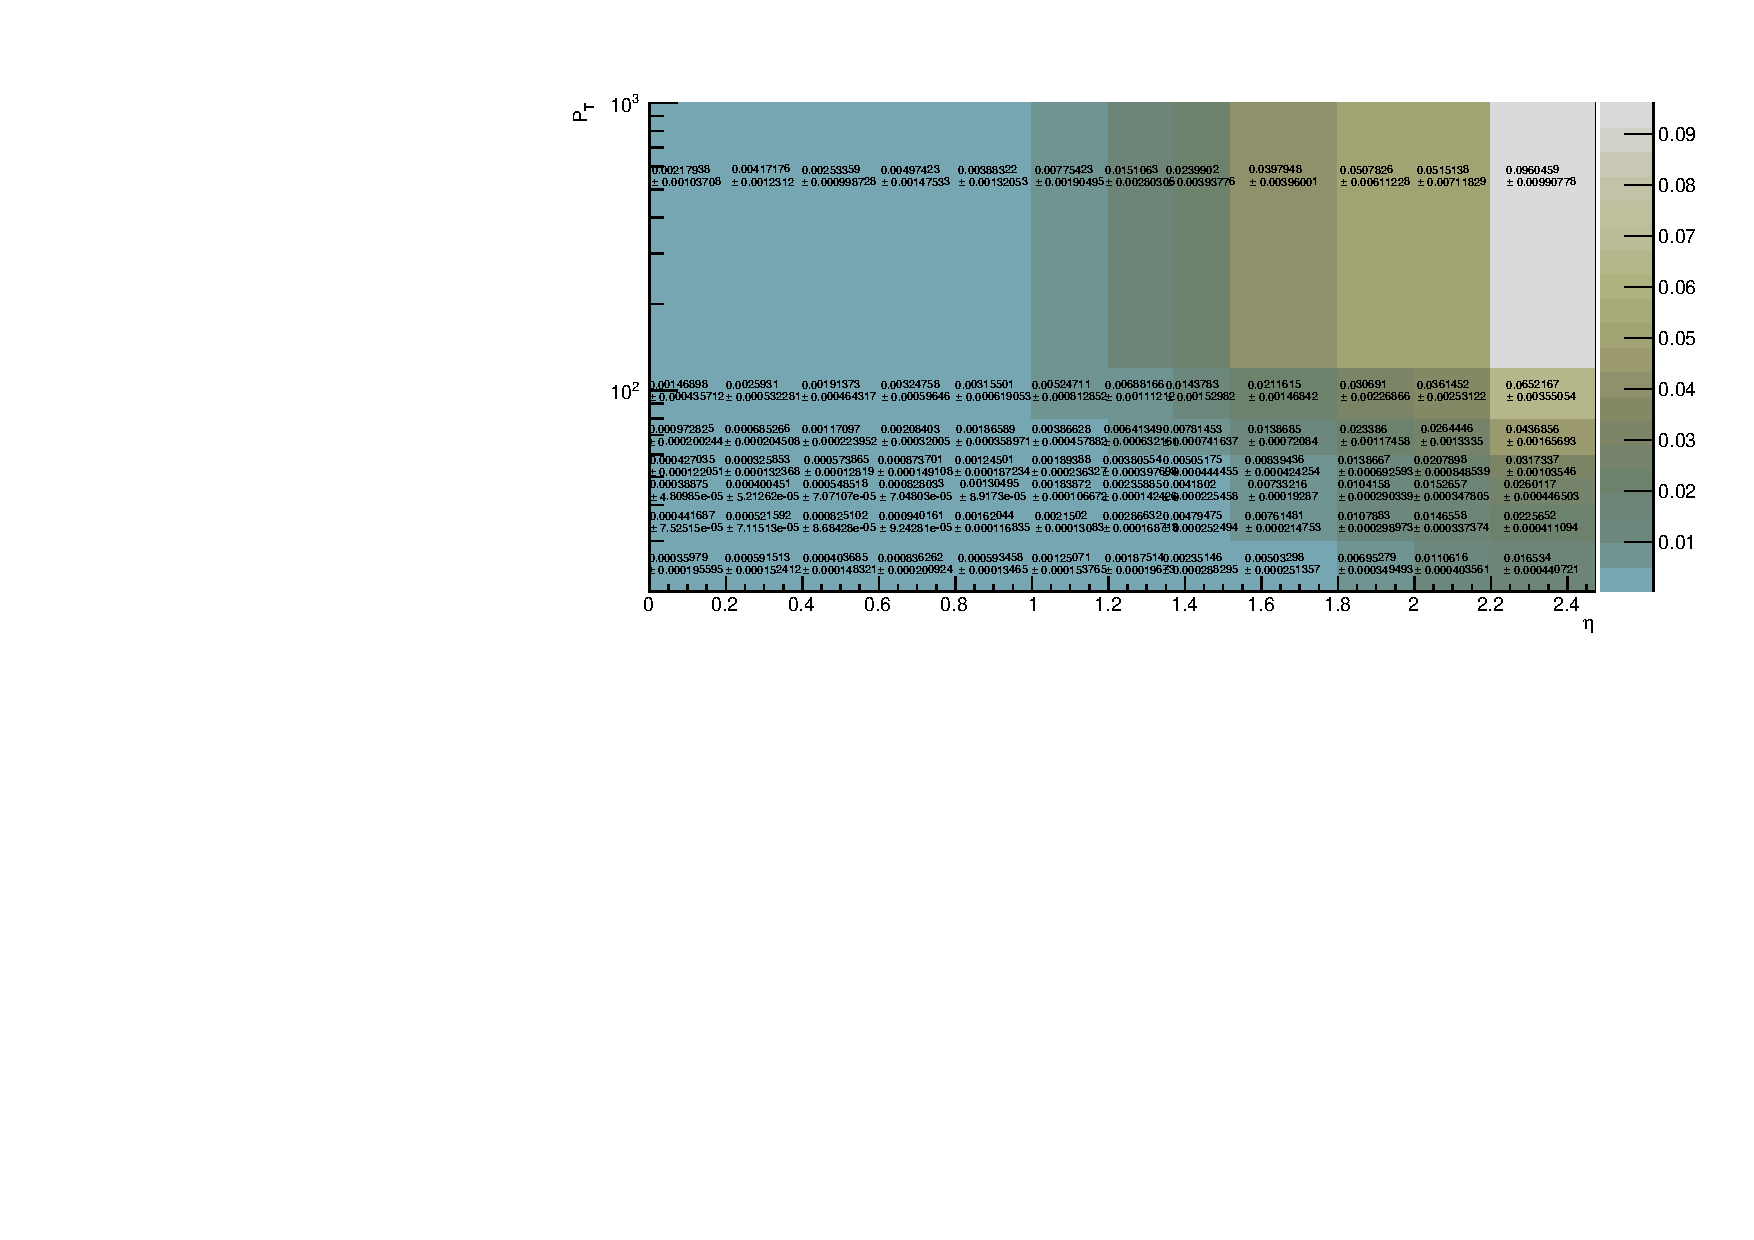
\includegraphics[width=\textwidth]{ChargeMisID/DataRates/DataLH.pdf}{}
\caption{Charge misidentification rates for Signal electrons in data with nominal Zmass window and sideband width}
\label{fig:DataRates2D}
\end{figure}

\FloatBarrier
\subsubsection*{Validation in data}
The rates were validated in the charge flip control region, defined by:

\begin{itemize}
\item $|m_{ee} - 91.2| < 10 [GeV]$
\item same-sign
\end{itemize}

Opposite sign events were weighted, as with the $Z\rightarrow ee$ sample to obtain an estimate of the charge flip background. 

$$p =(1-\epsilon_i)\epsilon_j + (1-\epsilon_j)\epsilon_i$$
$$w = \frac{p}{1-p}$$

Upon doing so, the distributions in figure \ref{DataDistNoPT} are obtained.

\begin{figure}[h]
\centering
\includegraphics[scale=0.4]{ChargeMisID/1115-DataNoPtCorr/hMass.pdf}
\includegraphics[scale=0.4]{ChargeMisID/1115-DataNoPtCorr/hPhi.pdf}\\
\includegraphics[scale=0.4]{ChargeMisID/1115-DataNoPtCorr/hLeadingPt.pdf}
\includegraphics[scale=0.4]{ChargeMisID/1115-DataNoPtCorr/hSubleadingPt.pdf}\\
\includegraphics[scale=0.4]{ChargeMisID/1115-DataNoPtCorr/hLeadingEta.pdf}
\includegraphics[scale=0.4]{ChargeMisID/1115-DataNoPtCorr/hSubleadingEta.pdf}
\caption{Observed vs predicted same-sign distributions in data}
\label{fig:DataDistNoPT}
\end{figure}

Applying the $\Delta p_T$ correction as in MC, we obtain figure \ref{fig:DataDistWPT}. Applying the \pT correction improves agreement

\begin{figure}[h]
\centering
\includegraphics[scale=0.4]{ChargeMisID/1031-DataPtCorr/hMass.pdf}
\includegraphics[scale=0.4]{ChargeMisID/1031-DataPtCorr/hPhi.pdf}\\
\includegraphics[scale=0.4]{ChargeMisID/1031-DataPtCorr/hLeadingPt.pdf}
\includegraphics[scale=0.4]{ChargeMisID/1031-DataPtCorr/hSubleadingPt.pdf}\\
\includegraphics[scale=0.4]{ChargeMisID/1031-DataPtCorr/hLeadingEta.pdf}
\includegraphics[scale=0.4]{ChargeMisID/1031-DataPtCorr/hSubleadingEta.pdf}
\caption{Observed vs predicted same-sign distributions in data with \pT correction}
\label{fig:DataDistWPT}
\end{figure}

\subsubsection*{Systematic uncertainties}

There are two main contributions to the systematic uncertainties. They are

\begin{enumerate}
\item Method bias (see figure \ref{fig:MCrates}), and.
\item selection of sidebands/Z mass window (figure \ref{fig:DataRates})
\end{enumerate}

For the first item, the uncertainty in each bin is taken to be the difference between the rates obtained in MC by the likelihood method and by MC truth. 

For the second item, the uncertainty in each bin is taken to be the difference between the nominal and the variation with the largest difference. 

The pythagorean sum of all uncertainties (since they are uncorrelated) are shown in figure \ref{fig:DataRatesWErr}.

\begin{figure}[h]
\centering
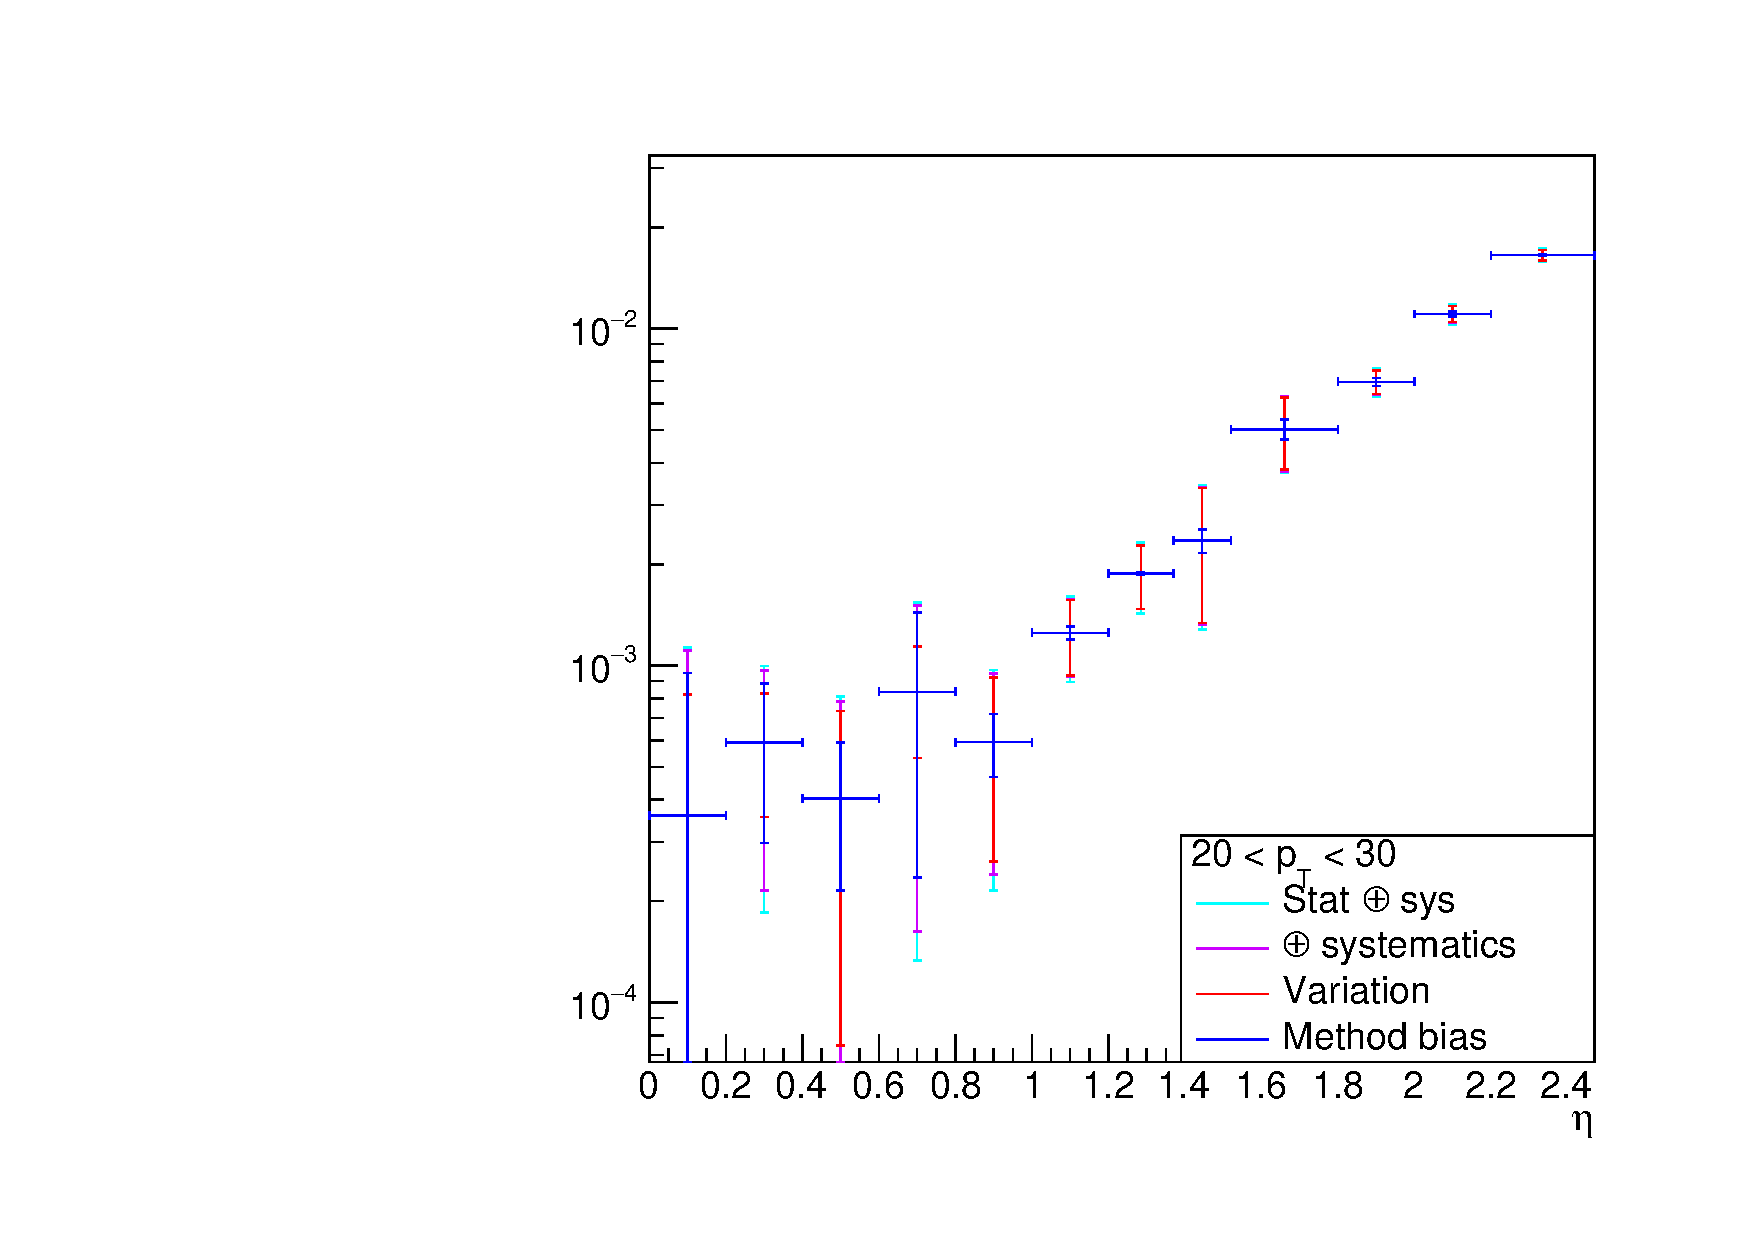
\includegraphics[page=1,scale=0.35]{ChargeMisID/dataRates/EtaPtErr.pdf}
\includegraphics[page=2,scale=0.35]{ChargeMisID/dataRates/EtaPtErr.pdf}\\
\includegraphics[page=3,scale=0.35]{ChargeMisID/dataRates/EtaPtErr.pdf}
\includegraphics[page=4,scale=0.35]{ChargeMisID/dataRates/EtaPtErr.pdf}\\
\includegraphics[page=5,scale=0.35]{ChargeMisID/dataRates/EtaPtErr.pdf}
\includegraphics[page=6,scale=0.35]{ChargeMisID/dataRates/EtaPtErr.pdf}
\phantomcaption
\end{figure}

\begin{figure}[h]
\ContinuedFloat
\centering
\includegraphics[page=7,scale=0.35]{ChargeMisID/dataRates/EtaPtErr.pdf}
\caption{Rates in data with all uncertainties}
\label{fig:DataRatesWErr}
\end{figure}

\FloatBarrier